\documentclass[twocolumn]{IEEEtran}
\usepackage{graphicx}
\usepackage[utf8x]{inputenc}
\usepackage{times}
\usepackage{amssymb,amsfonts}
\usepackage[tbtags]{amsmath}
\usepackage{cite}
\usepackage{pict2e}
\usepackage{float}
\usepackage{lscape}
\usepackage[all]{xy}
\usepackage{graphics,graphicx,color,colortbl}
\usepackage{times}
\usepackage{subfigure}
\usepackage{wrapfig}
\usepackage{multicol}
\usepackage{cite}
\usepackage{url}
\usepackage[tbtags]{amsmath}
\usepackage{amsmath,amssymb,amsfonts,amsbsy}
\usepackage{listings}
\usepackage{bm}
\usepackage{algorithm}
\usepackage{algorithmic}
\usepackage[centerlast, small]{caption}
\usepackage[colorlinks=true, citecolor=blue, linkcolor=blue, urlcolor=blue, breaklinks=true]{hyperref}
\hyphenation{ele-men-tos he-rra-mi-en-ta cons-tru-yen trans-fe-ren-ci-a pro-pu-es-tas si-mu-lar vi-sua-li-za-cion des-cri-ta co-rres-pon-dien-tes pro-ble-ma}

\begin{document}
\title{Propuesta: Enlace de Radio Frecuencia}
\author{David Ricardo Martínez Hernández Código: $261931$\\
	Jairo Andrés Neuta Bernal Código: $261227$\\
	Oscar Andres Urbano Vallejo Código: $261683$}
\maketitle
\markboth{Universidad Nacional de Colombia}{}
\floatname{algorithm}{Algoritmo}
\begin{keywords}
 ADC, Conversor, Comunicación inalámbrica, DAC, Línea de Transmisión, Microcinta, Modulador, Modulación ASK, Receptor, Transmisor.
\end{keywords}
\begin{abstract}
 En este documento se presenta la propuesta de metodología de diseño ,  haciendo énfasis en las etapas que se requiere para la comunicación digital ASK inalámbrica de una señal analógica, en el que se hará uso de diversas tapas en la que se sensará una señal analógica, se le hará su correspondiente acondicionamiento de señal para poder así ser manipulada digitalmente,  modulada y transmitida inalámbricamente a otro punto en donde luego de su recepción, su demodulación se acondicionara nuevamente la señal para ser leída e interpretada mediante un instrumento analógico. 
\end{abstract}

\section{Planteamiento del problema}
\noindent
Las comunicaciones inalámbricas han sido utilizas mucho en los últimos años para poder controlar o sensar algunas situaciones específicas, como lo es el control de temperatura de un lugar, también las comunicaciones de radio frecuencia como las estaciones de radio, de televisión análoga y hasta de comunicaciones celulares.\\
Para ello se quiere realizar el sensado de temperatura y poderla transmitir por medio del la modulación digital \textbf{ASK} a un galvanómetro. Para lograr esta modulación es necesario hacer uso de las herramientas adquiridas a lo largo de la carrera y así poder realizar dicha modulación con el mayor éxito posible.

\section{Objetivos}
\subsection{Objetivo General}
\begin{itemize}
 \item Realizar una comunicación ASK de una señal análoga y visualizarla en un galvanómetro.
\end{itemize}
\subsection{Objetivos Específicos}
\begin{itemize}
 \item Realizar la discretización de la señal análoga por medio de un conversor análogo digital (\textbf{ADC}).
 \item Realizar la conversión paralelo a serial de la señal análoga discretizada y la conversión serial paralelo de la misma señal.
 \item Realizar la modulación y demodulación de la señal que es transmitida por la antena.
 \item Realizar un acople de impedancias de todo el diseño a $50\Omega$.
 \item Realizar la construcción de la señal discreitzada a la señal original por medio de un conversor digital a análogo (\textbf{DAC}).
 \item Realizar un clock a $1KHz$ para sincronizar todos los dispositivos asíncronos.
\end{itemize}

\section{Diseño}
\noindent
El diseño se ha divido en dos etapas:
\begin{enumerate}
 \item Etapa de adquisición de datos, codificación y transmisión.
 \item Etapa de recepción, decodificación de datos y visua-lización.
\end{enumerate}
\noindent
La primera de estas etapas consta de cinco submodulos;  en esta subdivisón se encuentra el sensado de la señal analógica, posteriormente una etapa de amplificación y transducción de señal mediante un modulo \textbf{ADC} que muestrea, retiene, cuantifica y codifica la señal de interés, luego se tiene la etapa de de conversión  paralelo a serie de 8 bits, posterior a esto se encuentra la etapa de modulación por \textbf{ASK} para la transmisión y finalmente un modulo de acople mediante una linea de transmisión microcinta, con la antena transmisora (ver figura \ref{fig1}).\\
Con respecto a la segunda etapa principal, esta también cuenta con submodulos que la componen, de tal manera el proceso inverso al que se plantea desarrollar en la primera etapa, conforme a esto se tendría, una antena receptora acoplada a una linea microcinta, que a su vez  se comunicaría con el demodulador  seleccionado para esta aplicación,  posterior a esto la señal  demodulada pasara  por el modulo de conversión  de $8 bit$ serie a paralelo, luego se realiza  un proceso de  conversión digital análogo  de la señal tratada, por medio de un \textbf{DAC} y finalmente para efectos de manipulación y lectura de la señal analógica, se pasara la señal por un modulo de amplificación y visualización con galvanómetro (ver figura \ref{fig4}).

\subsection{Primera Etapa}

\begin{figure}[H]
	\centering
		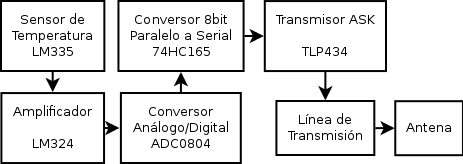
\includegraphics[scale=0.55]{Diagrama1.png}
	\caption{Etapa de adquisición de datos, codificación y transmisión.}
	\label{fig1}
\end{figure}

\subsubsection{Sensor de Temperatura}
\noindent
Como se observa en la Fig. \ref{fig1} la primera etapa empieza con la obtención de los datos de temperatura, esta se hará por medio del sensor de temperatura $LM335$, según la hoja de datos dicho sensor trabaja para valores de temperatura comprendidos entre $-40 ºC$ y $100 ºC$ estableciendo una diferencia de potencial entre sus terminales de $10 mV$ por cada $ºC$.\\ 
Según dicha información a la salida del sensor se tendrá un voltaje mínimo de $0 V$ para $-40 ºC$ y $1.4 V$ para $100 ºC$. Sin embargo el conversor \textbf{ADC} funciona para señales de entrada comprendidas entre $0V$ y $5V$ por tal motivo se propone una etapa de amplificación de la señal sensada.

\subsubsection{Amplificador de Voltaje}\label{amp}
\noindent
El amplificador de voltaje es un amplificador operacional $LM741$ o $LM324$, que contara con una relación de impedancias de $3.5$ para amplificar la señal  de entrada  de $0V -1.4 V$ a una señal de salida de $0V-5V$, esto con el fin de poseer una mejor resolución a la hora de convertir la señal análoga a digital, para mejores efectos prácticos se puede también hacer uso de un amplificador de instrumentación $AD6204$ que nos garantiza un alto rechazo al modo común y mejores condiciones de operación para la señal bajo ambientes de ruido. 

\subsubsection{Conversor Análogo Digital} \label{ADC}
El $ADC 0804$ (Fig. \ref{fig2}) puede ser alimentado con $5 V$, esto garantizara un muestreo óptimo para una señal de entrada análoga comprendida entre $0V - 5 V$, cuenta con una salida de $8$ bits lo cual da lugar a una definición de $256$ posibles valores, por lo cual con dicha polarización será capaz de detectar cambios a la entrada  hasta de $20mV$.
\begin{figure}[]
	\centering
		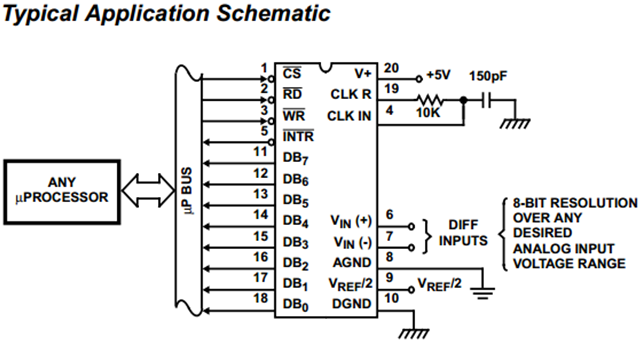
\includegraphics[scale=0.4]{ADC.png}
	\caption{Diagrama esquemático del $ADC0804$.}
	\label{fig2}
\end{figure}
\noindent
La tasa de conversión puede ser variada en función de los elementos conectados entre los pines  4 y 19 sin embargo para el montaje típico mostrado en la figura Fig. \ref{fig2} se cuenta con una Tasa de conversión de $f_{CLK} = 640kHz$.

\subsubsection{Conversor Paralelo Serial}
\noindent
Por medio del conversor $74HC175$ la señal obtenida del $ADC0804$ de $8$ bits es convertida a una señal serial de $1$ solo bit que contiene toda la información de los $8$ bits del \textit{ADC}. Este circuito es prácticamente un registro de desplazamiento,  funcionara con una señal de clock  de $1 KHz$ de frecuencia lo que hará que el bit serial que se transmita tenga una frecuencia de $1Kbps$,tasa de bits con la que funciona  el par transmisor receptor.  La señal de clock será suministrada por el circuito mostrado en la Fig. \ref{fig3} en el cual se utiliza el integrado $LM555$ para formar el oscilador.
\begin{figure}[H]
	\centering
		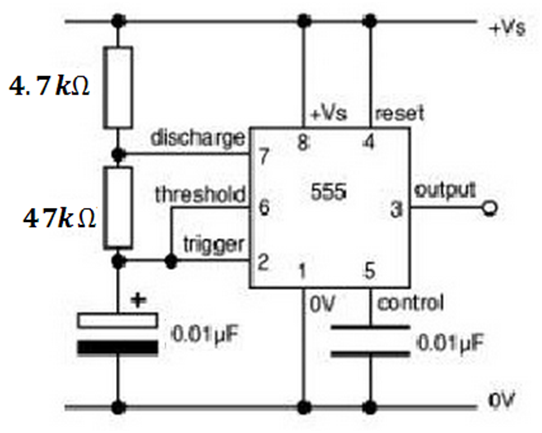
\includegraphics[scale=0.45]{555.png}
	\caption{Oscilador con el $LM555$.}
	\label{fig3}
\end{figure}

\subsubsection{Transmisor ASK}
\noindent
Para este caso se utilizara un $TLP434A$, el cual fue sugerido por el docente. Este transmisor es alimentado con $5 V$, opera con una tasa de bits de $1 Kbps$, este circuito se encarga de hacer la modulación y genera la onda que será llevada a la antena suministrada por el docente, esta referencia en específico modula la señal con una portadora de $434 MHz$, frecuencia central a la que será transmitida la información en el aire; se escogió el par transmisor receptor en esta frecuencia de operación ya que está comprendida en la banda destinada a los radio aficionados ($430 MHz – 440 MHz$).

\subsubsection{Línea de Transmisión} \label{LTx}
\noindent
Como es necesario utilizar una línea de transmisión para realizar las conexiones correspondientes se utilizo un arreglo de líneas para poder acoplar la unión del modulador con la antena, este acople debe estar diseñado a $50\Omega$ porque todos los elementos del circuito también lo están.\\
Se utilizaron dos líneas de microcinta acopladas, la primera tiene una longitud de $l_1=97.5733mm$, un ancho de $w_1=4.5mm$, asumiendo un $\epsilon _R = 3.7$, espesor del dieléctrico de $H=0.711mm$, y un ancho de la pista de cobre de $T=35 \mu m$.\\
Para la segunda línea de transmisión que tiene las mismas características $\epsilon _R$, $H$ y $T$ iguales, se obtuvo un largo de $l_2=99.9294mm$ y un ancho de $w_2=2.70175mm$.\\
Estos resultados se obtuvieron con el simulador \textbf{Qucs $0.0.16$}.

\subsubsection{Antena}
\noindent
Suministrada por el docente, se sabe que tiene una impedancia de $50 \Omega$.

\subsection{Segunda Etapa}
\begin{figure}[H]
	\centering
		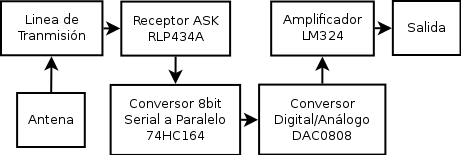
\includegraphics[scale=0.55]{Diagrama2.png}
	\caption{Etapa de recepción, decodificación de datos y visualización.}
	\label{fig4}
\end{figure}

\subsubsection{Antena}
\noindent
Suministrada por el docente, se sabe que tiene una impedancia de $50 \Omega$.

\subsubsection{Línea de Transmisión}
\noindent
Se utilizará la misma linea descrita en la etapa anterior (ver  ~\ref{LTx}).

\subsubsection{Demodulador ASK}
\noindent
Se utilizará el receptor $RLP434$ que es el receptor compatible con el transmisor $TLP434A$. Trabaja a la misma frecuencia de operación ($434 MHz$) y con la misma tasa de bits ($1Kbps$), el receptor además demodula la señal y entrega el bit serial que contiene la información de la temperatura.

\subsubsection{Conversor Serial Paralelo}
\noindent
Se utilizará el conversor Serial Paralelo $74HC164$. Que trabajara a la misma frecuencia de operación que el $ADC$ (ver  ~\ref{ADC})) utilizado en la primera etapa de diseño, por tanto utilizara el mismo circuito de la Fig. \ref{fig3} para obtener la señal de clock de $1KHz$.

\subsubsection{Conversor Digital Análogo}
\noindent
Se utilizará el conversor Digital-Análogo $DAC0808$.

\subsubsection{Amplificador de Voltaje}
\noindent
Como se tiene el mismo problema que en la sección anterior se realizara la misma o-peración tratando de igualar el voltaje máximo a $5V$ (ver  ~\ref{amp}).

\subsubsection{Salida}
\noindent
Se utilizara un galvanómetro suministrado por el docente.

\section{Costos}
\noindent
Para realizar este proyecto se van a utilizar estos recursos:
\begin{table}[H]
	\centering
\begin{tabular}{|c|c|r|r|}\hline
 \textbf{Cantidad} & \textbf{Recurso} & \textbf{Valor Unitario} & \textbf{Total} \\ \hline
 1 & Sensor $LM335$ & $1.800$ & $1.800$ \\ \hline
 2 & Amplificadores $LM324$ o $LM741$ & $800$ & $1.600$ \\ \hline
 1 & $ADC0804$ & $8.700$ & $8.700$ \\ \hline
 1 & $74HC165$ & $1.000$ & $1.000$ \\ \hline
 2 & $LM555$ & $550$ & $1.100$ \\ \hline
 1 & $TLP434A$ & $9.300$ & $9.300$ \\ \hline
 1 & $RLP434$ & $10.100$ & $10.100$ \\ \hline
 1 & $74HC164$ & $700$ & $700$ \\ \hline
 1 & $DAC0808$ & $4.350$ & $4.350$ \\ \hline
 2 & Circuito Impreso de $20cm*20cm$ & $3.000$ & $6.000$ \\ \hline
    \end{tabular}
	\caption{Costos de implementación.}
	\label{tab1}
\end{table}
\noindent
Para realizar este proyecto es necesario hacer una inversión de aproximadamente $\$ 57.750$, sin tomar en cuenta las horas de diseño por cada integrante del grupo.

\bibliographystyle{ieeetran}
\begin{thebibliography}{99}

\bibitem{balanice} Balanice, Constantine A.
{\em ``Antenna theory analysis and desing''}.
John Wiley \& Sons, Inc., Third Edition, 2005

\bibitem{pozar} Pozar, David M.
{\em ``Microwave Engineering''}.
John Wiley \& Sons, Inc., Fourth Edition, 2012

\bibitem{page0} Sitio web: \url{http://www.sigmaelectronica.net}, visitado el 04 de junio de 2013.

\bibitem{page00} Sitio web: \url{http://www.tekcien.com}, visitado el 04 de junio de 2013.

\bibitem{page1} Hoja de datos del $LM335$: \url{http://www.sigmaelectronica.net/manuals/LM335.pdf}, leída el 04 de junio de 2013.

\bibitem{page2} Hoja de datos del $LM324$: \url{http://www.sigmaelectronica.net/manuals/LM324.pdf}, leída el 04 de junio de 2013.

\bibitem{page3} Hoja de datos del $LM741$:\url{http://www.sigmaelectronica.net/manuals/LM741.pdf}, leída el 04 de junio de 2013.

\bibitem{page4} Hoja de datos del $ADC0804$: \url{http://www.sigmaelectronica.net/manuals/ADC0804.pdf}, leída el 04 de junio de 2013.

\bibitem{page5} Hoja de datos del $74HC165$: \url{http://www.sigmaelectronica.net/manuals/74HC165.pdf}, leída el 04 de junio de 2013.

\bibitem{page5} Hoja de datos del $LM555$: \url{http://www.sigmaelectronica.net/manuals/LM555.pdf}, leída el 04 de junio de 2013.

\bibitem{page6} Hoja de datos del $TLP434A$: \url{http://www.sigmaelectronica.net/manuals/TLPRLP434A.pdf}, leída el 04 de junio de 2013.

\bibitem{page7} Hoja de datos del $RLP434$: \url{http://www.sigmaelectronica.net/manuals/tlprlp434.pdf}, leída el 04 de junio de 2013.

\bibitem{page8} Hoja de datos del $74HC164$: \url{http://www.sigmaelectronica.net/manuals/74HC164.pdf}, leída el 04 de junio de 2013.

\bibitem{page9} Hoja de datos del $DAC0808$: \url{http://www.sigmaelectronica.net/manuals/DAC0808.pdf}, leída el 04 de junio de 2013.

\bibitem{page10} Sitio web: \url{http://www.microelectronicos.com/datasheets/MO-RX3400.pdf}, visitado el 04 de junio de 2013.

\bibitem{page11} Sitio web: \url{http://www.microelectronicos.com/datasheets/MO-SAWR.pdf}, visitado el 04 de junio de 2013.

\end{thebibliography}
\end{document}